\chapter{Ziel}
\label{chap:software-design}
In diesem Kapitel wird ein mögliches Design für den RoboCup erläutert.
\section{Einführung}
In den nachfolgenden Abschnitten soll gezeigt werden, wie man die einzelnen Systeme des Roboters in Services (Positionierung, Drive-Einheit, Greifsystem, etc.) unterteilt und dazwischen simple Schnittstellen realisieren kann.
Jede einzelne Komponente im System verwendet zum Austausch mit Anderen den Systemweiten Message Broker.

\section{Monolith vs. Microservice}
Man hört es heute an jedem Entwickler-Event, liest es in verschiedenen Zeitschriften, egal ob für Entwickler oder System-Administratoren: der Weg zum Ziel sollen Microservices sein, sie sollen Monolithen ablösen. Viele kleine Services statt einen grossen, verzahnten und schwierig wartbaren Moloch.
In \cite{informatik-aktuell-microservices} findet sich ein passendes Statement zur monolithischen Applikation:
\begin{formal}
	Selbstverständlich startet keine Neuentwicklung als ,,grosser Monolith". Anfangs ist die Anwendung schlank, leicht zu erweitern und gut zu verstehen – die Architektur adressiert die Probleme, die das Team zu dieser Zeit hat. Im Laufe der Monate entsteht mehr und mehr Code. Es werden Schichten definiert, Abstraktionen gefunden, Module, Services und Frameworks eingeführt, um die wachsende Komplexität in den Griff zu bekommen.
	
	Bereits bei mittelgrossen Anwendungen (etwa eine Java-Anwendung mit mehr als 50.000 LOC\footnote{Lines of Code}) werden monolithische Architekturen langsam unangenehm. Das gilt vor allem für Anwendungen, die hohe Anforderungen an die Skalierbarkeit stellen. Aus der schlanken Neuentwicklung entwickelt sich das nächste Legacy-System, über das folgende Generationen von Entwicklern fluchen werden.
\end{formal}
\subsection{Vorteile von Microservices}
Die Vorteile von Microservices sprechen für sich. Deshalb setzen auch die Internetriesen wie Netflix, Amazon, eBay und Uber seit einiger Zeit darauf. Hier ein Auszug der wichtigsten Punke aus der selben Quelle\cite{informatik-aktuell-microservices}, die für den Roboter interessant sind:
\begin{formal}
	\begin{itemize}
		\item
		Aufgrund ihrer geringen Grösse benötigt man wenig Boiler-Plate Code und keine schwergewichtigen Frameworks.
		\item
		Sie lassen sich unabhängig voneinander deployen. Continuous Delivery bzw. Deployment lässt sich damit sehr viel einfacher realisieren.
		\item
		Die Architektur unterstützt die Arbeit in mehreren, unabhängigen Teams.
		\item
		Es ist pro Service möglich, die jeweils „beste“ Programmiersprache zu wählen. Man kann ohne grosses Risiko auch mal eine neue Sprache, ein neues Framework oder ähnliches ausprobieren. Man sollte es dabei nur nicht übertreiben.
		\item
		Da sie klein sind, lassen sie sich auch jederzeit mit vertretbarem Aufwand durch eine Neuentwicklung ablösen.
		\item
		Microservices kommen der agilen Entwicklung entgegen. Ein neues Feature, von dessen Erfolg beim Kunden man noch nicht überzeugt ist, lässt sich nicht nur schnell entwickeln – es lässt sich auch schnell wieder wegwerfen.
	\end{itemize}
\end{formal}

Folgendes Argument kommt noch dazu: Durch die Tatsache, dass die Schnittstellen klar definiert sind, lassen sich an einem Service jederzeit einfache Blackbox-Tests durchführen: Man versorgt den Service an der Schnittstelle mit den Testdaten und prüft, ob die richtigen Daten raus kommen. Diesen Punkt werden wir später in diesem Dokument anhand des \acrshort{lidar}-Services anschauen.
\subsection{Nachteile von Microservices}
Natürlich gibt es mit Microservices auch Nachteile, die man nicht verschweigen sollte:
\begin{itemize}
	\item
	Durch die Kapselung in einzelne Komponenten (und sogar eigene Java VMs) braucht es  grundsätzlich mehr Ressourcen. Vor allem in Bezug auf Memory und Netzwerkverkehr.
	\item
	Objekte werden in einer YAML-/JSON-/(XML)-Struktur serialisiert übers Netzwerk versendet. Der Consumer-Service muss diese dann wieder in Objekte ,,abfüllen'' (marshalling/unmarshalling). Dieses Serialisieren und Deserialisieren ist ziemlich ,,teuer'' was die CPU Performance anbelangt.
	
\end{itemize}


\section{Architektur}
\label{sec:Architektur}
Das historisch gewachsene, monolithische Design (Schaubild \ref{fig:architecture_current_highlevel}) soll also umgebaut werden.
\begin{figure}[H]
	\centering
	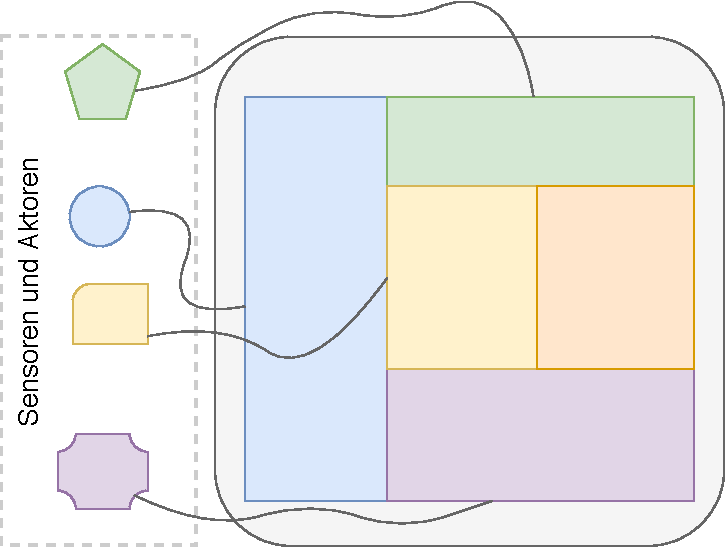
\includegraphics[width=0.3\textwidth]{img/architecture-highlevel-today.pdf}
	\caption{Bestehende Architektur (plakatives Schaubild)}
	\label{fig:architecture_current_highlevel}
\end{figure}
Beim bestehenden Design kommunizieren einige Komponenten bereits heute über das \acrshort{mqtt}-Protokoll (Details zu \acrshort{mqtt} im Abschnitt \ref{sec:mqtt}). In der neuen Architektur soll dies komplett in den Mittelpunkt rücken und für den Datenaustausch der einzelnen Services zuständig sein. Es gäbe auch andere Event-/Message-Busse, die dafür verwendet werden könnten (Bsp. \Gls{ros}). In Diskussionen mit dem Betreuer und dem Auftraggeber hat sich aber herausgestellt, dass \Gls{ros} zu viele Herausforderungen mit sich bringt. ,,Das RoboCup-Team aus Deutschland beisse sich daran auch die Zähne aus.'' \\
\acrshort{mqtt} ist durch die Verwendung in Heimautomationen bereits weit verbreitet und es gibt Libraries für unterschiedliche Programmiersprachen und eine grosse Community dafür. Vor allem aber kennen die Studenten der HFTM dieses Protokoll bereits. \\ Es sollen also Microservices entstehen, die nur genau eine Aufgabe erfüllen. Einige werden nur das hardware-spezifische Protokoll (hier \acrshort{lidar}) in die \acrshort{mqtt}-Welt adaptieren. Andere werden Berechnungen mit den Daten ausführen und die Resultate wieder bereitstellen. \Glspl{service} kennen sich untereinander nicht, sie wissen nichts von der Existenz anderer \glspl{service}. Damit die einzelnen \Glspl{service} miteinander kommunizieren können, kommen Verbinder zum Einsatz,  so genannte \Glspl{servant}. Diese kennen die Schnittstellen (\gls{contract} bzw. \acrshort{api}) der zu bedienenden Services. Wir werden dieses Konzept in den nachfolgenden Kapitel am Beispiel des \acrshort{lidar} anschauen.

\begin{figure}[H]
	\centering
	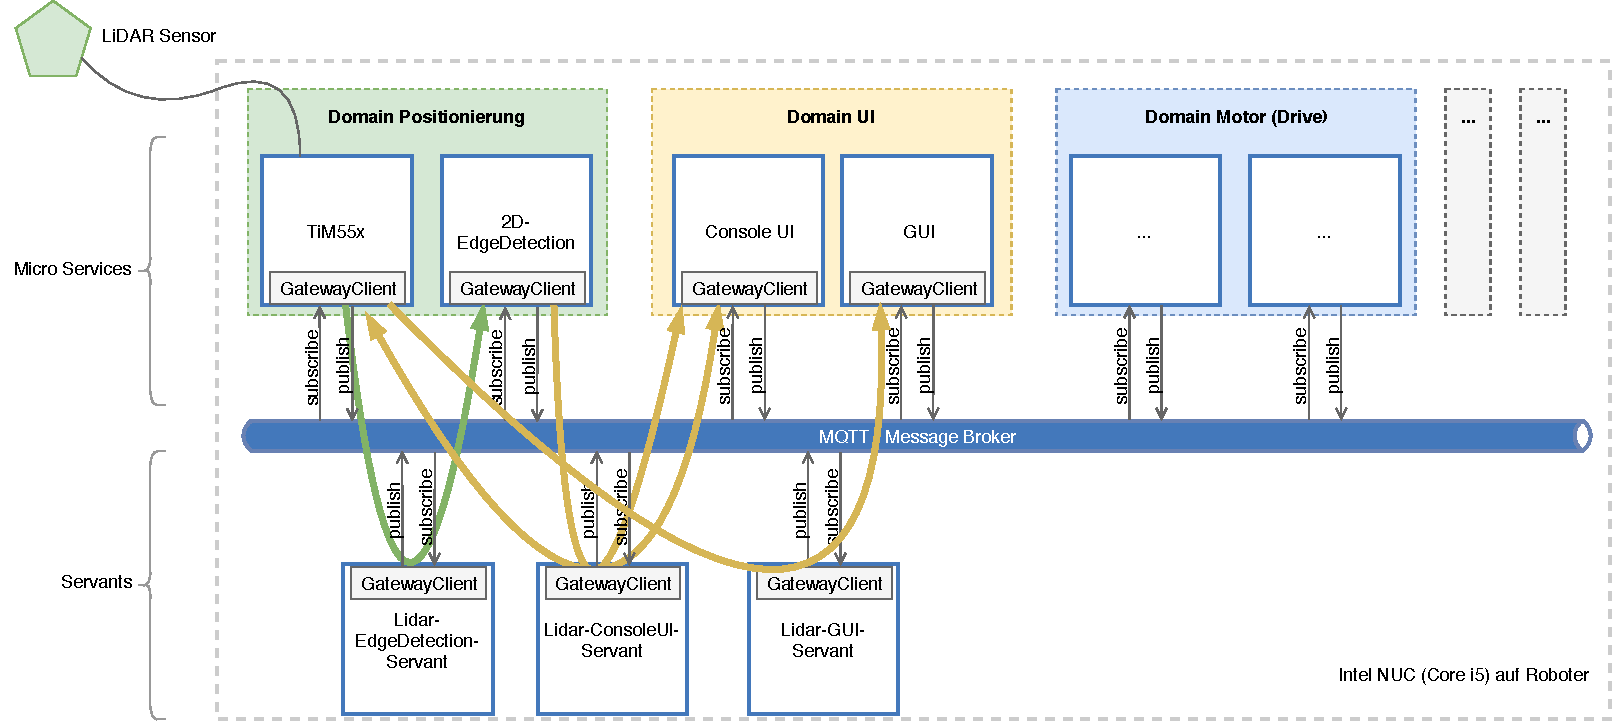
\includegraphics[width=\textwidth]{img/architecture-highlevel.pdf}
	\caption{Architektur in Domains}
	\label{fig:architecture_highlevel}
\end{figure}

Die Abbildung \ref{fig:architecture_highlevel} zeigt wie die einzelnen Services durch die Servants verbunden werden. Ein Servant kann mehrere Services ,,verbinden'' dafür gibt es keine Regel. Es gibt beispielsweise einen \Gls{servant}, der die gelieferten Daten vom TiM55x-Service konvertiert und dem EdgeDetection-Service gibt. Fürs UI könnten aber sowohl Daten vom TiM55x-Service als auch vom EdgeDetection-Service relevant sein. Dazu wird der \acrshort{lidar}-UI-Servant die Daten entsprechend zusammenführen und dem UI-Service übergeben. Der UI-Service dient hier nur als Beispiel. In der Praxis - also im Kontext des RoboCups - werden diese Informationen vielleicht an einem Service mit Fahrlogik übergeben.

\subsection{Ausführung der Services, Hardware-Ressourcen}
Die Idee ist grundsätzlich, dass jeder Service für sich ausgeführt wird. Im Kontext der nach diesem Leitfaden entwickelten Services bedeutet das aber, dass für jeden Service eine eigene Java VM gestartet wird. Je nach Anzahl der Services wird auf der Zielplattform, dem Intel NUC, aber zu wenig Arbeitsspeicher für dieses Vorhaben zur Verfügung stehen. Deshalb ist vorgesehen, dass es pro Domäne einen 'Domänen-Runner' gibt, der alle Services einer Domäne in einer JVM startet.

\section{Aufbau eines Services, Begriffe}
\label{sec:isePattern}
Jeder Service im System soll sich an in diesem Abschnitt beschriebenen Grundsatz halten. Als Student der BFH mit Mobile Computing als Schwerpunkt lernt man bei Reto Koenig folgendes Muster für die MQTT-Topics kennen: Intent, Status und Event. Was das bedeutet wird in den nächsten Abschnitten beschrieben. Die \acrshort{mqtt}-Topics stellen das \acrshort{api} für den jeweiligen Service dar. \\ Die nachfolgenden Teilabschnitte basieren auf dem englischen README aus dem Github-Projekt von Reto Koenig \cite{ch.quantasy.mqtt.gateway}.

\subsection{Payload}
In der Payload der Topics - also der Nachricht - befindet sich nicht nur ein Wert wie bisher, sondern eine Struktur (JSON, YAML, XML, etc.). Wir verwenden hier \acrshort{yaml}, damit man die Daten mit einem handelsüblichen MQTT-Client (z.B. MQTTlens\cite{mqtt-lens} oder MQTTfx\cite{mqttfx}) für den Mensch sehr einfach verständlich anzeigen kann (siehe Listing \ref{lst:examplePayload}). Denn \acrshort{yaml} ist frei von eckigen, spitzigen und runden Klammern, Tags und Kommas. Jede Payload enthält mindestens einen Zeitstempel mit der Systemzeit als die Meldung ins MQTT-System eingespiesen wurde. Der Zeitstempel einer Nachricht von einem Service wird bei Bedarf vom Servant ausgewertet und je nach Anwendungsfall weiterverarbeitet.

\begin{lstlisting}[caption={Beispiel einer MQTT-Payload}, label={lst:examplePayload}]
---
- timeStamp: 65630678285913
  command: "SINGLE_MEASUREMENT"
\end{lstlisting}

\subsection{Unit}
Als \gls{unit} wir eine Instanz eines Services bezeichnet. Beispielsweise wird der TiM55x-Service für jeden vorhandenen \acrshort{lidar}-Sensor als eine individuelle Instanz gestartet. Das sind also unterschiedliche Units. Jede Instanz bzw. Unit hat sein eigenes MQTT Basis-Topic.

\subsection{Intent}
Kann ein Service Befehle über die \acrshort{mqtt}-\acrshort{api} entgegennehmen, so werden diese über das Topic '\gls{intent}' dem Service mitgeteilt. Dafür muss sich der Service auf dieses Topic abonnieren ('subscribe'). Pro Service gibt es nur ein Intent-Topic. \\ Es hat sich herausgestellt, dass ein Design mit mehreren Intent-Topics pro Services unpraktikabel ist. Beispielsweise sind sie plötzlich abhängig untereinander, dh. es muss zuerst das eine Intent und später das andere gesendet werden. Das ist fast nicht handhabbar wenn verschiedene Teilnehmer mit einem Service interagieren. Ein ähnliches Konzept verfolgt auch Google bei Android. Zuerst wird der komplette Intent definiert (also die Absicht was das System tun soll und wie) und dann wird er versendet.

\subsection{Status}
Mehrheitlich statische Informationen stellt ein Service unter dem Basis-Topic '\gls{status}' zur Verfügung. Am Beispiel des \acrshort{lidar}-Sensors gehören hier jegliche Informationen über den Sensor in diese Kategorie rein: Firmwarestand, Konfiguration, State des Sensors (Sensor wird initialisiert / Messung läuft / Standby / etc.). Unter diesem Topic kann eine beliebige Baumstruktur aufgebaut werden.

\subsection{Event}
Alle Informationen, die eventgesteuert sind oder auftreten können, klassifizieren wir in diese Kategorie. Die Messwerte des Sensors gehören beispielsweise in dieses Topic.

\subsection{Description}
Im Topic '\gls{description}' beschreibt ein Service bzw. eine \acrshort{unit} beim Aufstarten das angebotene \acrshort{api}. Das ermöglicht für Entwickler die Anbindung an andere Komponenten. Die Description des APIs ist vor allem für die Entwicklung von Services relevant, die nicht den im nachfolgenden Kapitel beschriebenen \ctexttt{GatewayClient} verwenden.

\subsection{Beispiele}
Ein Topic in unserem sieht also Beispielsweise wie folgt aus:

\begin{minipage}{\linewidth}
\begin{verbatim}
Robocup/Lidar/U/192.168.91.2@kicm-fedora.localdomain/S/connection
         ^    ^       ^                              ^  ^
         |    |       |                              |  |
         |    |       |                              |  '--- Topic unterhalb 'Status'
         |    |       |                              '------ Status Trennzeichen
         |    |       '------------------------------------- Name der Unit / Instanz
         |    '--------------------------------------------- Unit Trennzeichen
         '-------------------------------------------------- Name des Services
\end{verbatim}
\end{minipage}

\subsubsection{Beispiel mehrere \acrshort{lidar}-Sensoren}
Wenn wir mehrere Sensoren verwenden, arbeiten die Instanzen des TiM55x-Services beispielsweise in diesen Basis-Topics:
\begin{itemize}
	\item \texttt{Robocup/Lidar/U/192.168.91.11@mainpc.robot1.hftm.localdomain/...}
	\item \texttt{Robocup/Lidar/U/192.168.91.22@mainpc.robot1.hftm.localdomain/...}
	\item \texttt{Robocup/Lidar/U/192.168.91.33@mainpc.robot1.hftm.localdomain/...}
\end{itemize}

\subsubsection{Beispiel \acrshort{lidar}-Sensoren auf einem Roboter verteilt auf mehrere Computer}
Wenn wir mehrere Sensoren verwenden, arbeiten die Instanzen des TiM55x-Services beispielsweise in diesen Basis-Topics:
\begin{itemize}
	\item \texttt{Robocup/Lidar/U/192.168.91.11@mainpc.robot1.hftm.localdomain/...}
	\item \texttt{Robocup/Lidar/U/192.168.91.22@secondpc.robot1.hftm.localdomain/...}
	\item \texttt{Robocup/Lidar/U/192.168.91.33@secondpc.robot1.hftm.localdomain/...}
\end{itemize}